\documentclass{report}  
\usepackage[utopia]{mathdesign} 
%\usepackage{amsmath,amsfonts,amsthm,amssymb,mathtools}

\usepackage[french]{babel}
%\usepackage[utopia]{mathdesign}

% Permet d'ajuster la taille des marges et de la distance pour les footer
\usepackage[tmargin=2cm,rmargin=0.4in,lmargin=0.4in,bmargin=2cm,footskip=.2in]{geometry}

% Permet d'optimiser l'affichage de différents symboles et formules mathématiques
%\usepackage{amsmath,amsthm,mathtools}
%usepackage{amsmath,amsfonts,amsthm,amssymb,mathtools}

\usepackage{svg}
% Modifie l'apparence des nombre en mathmode et textmode
%\usepackage[varbb]{newpxmath}

% Modifier l'apparence des fractions
\usepackage{xfrac}

            %%%%%%%%%%%%%%%%%  Sect.        14 Oct 2024     %%%%%%%%%%%%%%%%%%%%%%%%%%%%%%%%%%%%%%%%%%%%%%%%%%%%%%%%%%%
\usepackage{graphicx}
\usepackage{caption}
\usepackage{subcaption}
\usepackage{arydshln}
            %%%%%%%%%%%%%%%%%  Sect.        14 Oct 2024     %%%%%%%%%%%%%%%%%%%%%%%%%%%%%%%%%%%%%%%%%%%%%%%%%%%%%%%%%%%
\usepackage{balance}
\usepackage{dirtree}
\usepackage{titlesec}






% Permet de rayer (barrer) l'argument avec la touche
% \cancel{} \bcancel{} ou \xcancel{}
\usepackage[makeroom]{cancel}

% Extension du package amsmath; corrige certains bugs et déficiences de son prédecesseur
%\usepackage{mathtools}

% This package provides most of the flexibility you may want to customize the three basic list
% environments (enumerate, itemize and description)
\usepackage{bookmark} 

% Réorganiser les théorèmes et Lemmes. Usage complexe. 
% Référence : https://ctan.math.illinois.edu/macros/latex/contrib/theoremref/theoremref-doc.pdf
\hypersetup{hidelinks}
\usepackage{hyperref,theoremref} 

% Fournit un environnement pour créer des boîtes colorées
\usepackage[most,many,breakable]{tcolorbox}


%\newcommand\mycommfont[1]{\footnotesize\ttfamily\textcolor{blue}{#1}}\SetCommentSty{mycommfont}

%\newcommand{\incfig}[1]{%\def\svgwidth{\columnwidth}\import{./figures/}{#1.pdf_tex}}
\newcommand{\arc}[1]{\wideparen{#1}}

%Pour colorer les lignes séparatrices de tableaux
\usepackage{colortbl}
\usepackage{tikzsymbols}

\usepackage{framed}
\usepackage{titletoc}
\usepackage{etoolbox}
\usepackage{lmodern}
\usepackage{tabularx}
\usepackage{enumitem}
\usepackage{amsthm}
            %%%%%%%%%%%%%%%%%  Sect.        14 Oct 2024     %%%%%%%%%%%%%%%%%%%%%%%%%%%%%%%%%%%%%%%%%%%%%%%%%%%%%%%%%%%

\usepackage{lipsum}
\usepackage{titling}
\renewcommand\maketitlehooka{\null\mbox{}\vfill}
\renewcommand\maketitlehookd{\vfill\null}

\newcommand{\varitem}[3][black]{%
  \item[%
   \colorbox{#2}{\textcolor{#1}{\makebox(5.5,7){#3}}}%
  ]
}
\usepackage{afterpage}
\newcommand\myemptypage{
    \null
    \thispagestyle{empty}
    \addtocounter{page}{-1}
    \newpage
    }




% from https://tex.stackexchange.com/a/167024/121799
\newcommand{\ClaudioList}{red,DarkOrange1,Goldenrod1,Green3,blue!50!cyan,DarkOrchid2}
\newcommand{\SebastianoItem}[1]{\foreach \X[count=\Y] in \ClaudioList
{\ifnum\Y=#1\relax
\xdef\SebastianoColor{\X}
\fi
}
\tikz[baseline=(SebastianoItem.base),remember
picture]{%
\node[fill=\SebastianoColor,inner sep=4pt,font=\sffamily,fill opacity=0.5] (SebastianoItem){#1)};}
}
\newcommand{\SebastianoHighlight}{\tikz[overlay,remember picture]{%
\fill[\SebastianoColor,fill opacity=0.5] ([yshift=4pt,xshift=-\pgflinewidth]SebastianoItem.east) -- ++(4pt,-4pt)
-- ++(-4pt,-4pt) -- cycle;
}}   
            %%%%%%%%%%%%%%%%%  Sect.        14 Oct 2024     %%%%%%%%%%%%%%%%%%%%%%%%%%%%%%%%%%%%%%%%%%%%%%%%%%%%%%%%%%%





%====================================================================

%====================================================================
\newcommand*{\authorimg}[1]%
    { \raisebox{-1\baselineskip}{\includegraphics[width=\imagesize]{#1}}}
\newlength\imagesize  

\usepackage{pgfplots}
\pgfplotsset{compat=1.17}

%==========================================================================================
\usepackage{libris} 
\usepackage{etoolbox}
\usepackage[export]{adjustbox}% for positioning figures

\makeatletter
% Force le chapitre suivant sur la ligne succedant la fin du 
% chapitre précédent
\patchcmd{\chapter}{\if@openright\cleardoublepage\else\clearpage\fi}{}{}{}
\makeatother
\usepackage[Sonny]{fncychap}


%boîte de couleur grise
\tcbset{
  graybox/.style={
    colback=gray!20,
    colframe=black,
    sharp corners=downhill,
    boxrule=1pt,
    left=5pt,
    right=5pt,
    top=5pt,
    bottom=5pt,
    boxsep=0pt,
	 % <-- add four values for each corner
  }
}
\newtcolorbox{graybox}{graybox}

%==========================================================================================



\usepackage{xcolor}
\usepackage{varwidth}
\usepackage{varwidth}
\usepackage{etoolbox}
%\usepackage{authblk}
\usepackage{nameref}
\usepackage{multicol,array}
\usepackage{tikz-cd}
\usepackage[ruled,linesnumbered,ruled]{algorithm2e}
\usepackage{comment} % enables the use of multi-line comments (\ifx \fi) 
\usepackage{import}
\usepackage{xifthen}
\usepackage{pdfpages}
\usepackage{transparent}


%\usepackage[french]{babel}
\usepackage{listings} % pour écrire du code dans un environnement
\lstset{
  basicstyle=\ttfamily,
  columns=fullflexible,
  keepspaces=true
}
\usepackage{caption}
\usepackage{float} % Pour forcer les images au bon endroit



\usepackage[T1]{fontenc}
\usepackage{csquotes}
%%%%%%%%%%%%%%%%%%%%%%%%%%%%%%%%%%%%%%%%%%%%%%%%%%%%%%%%%%%%%%%%%%%%%%%%%%%%%%%%%%%%%%%%%%%%%%%%%
%									ENSEMBLE DE COULEURS
%%%%%%%%%%%%%%%%%%%%%%%%%%%%%%%%%%%%%%%%%%%%%%%%%%%%%%%%%%%%%%%%%%%%%%%%%%%%%%%%%%%%%%%%%%%%%%%%%

\definecolor{myg}{RGB}{56, 140, 70}
\definecolor{myb}{RGB}{45, 111, 177}

\definecolor{mygbg}{RGB}{235, 253, 241}


\definecolor{myr}{RGB}{199, 68, 64}
\definecolor{mytheorembg}{HTML}{F2F2F9}
\definecolor{mytheoremfr}{HTML}{00007B}
\definecolor{mylenmabg}{HTML}{FFFAF8}
\definecolor{mylenmafr}{HTML}{983b0f}
\definecolor{mypropbg}{HTML}{f2fbfc}
\definecolor{mypropfr}{HTML}{191971}
\definecolor{myexamplebg}{HTML}{F2FBF8}
\definecolor{myexamplefr}{HTML}{88D6D1}
\definecolor{myexampleti}{HTML}{2A7F7F}
\definecolor{mydefinitbg}{HTML}{E5E5FF}
\definecolor{mydefinitfr}{HTML}{3F3FA3}
\definecolor{notesgreen}{RGB}{0,162,0}
\definecolor{myp}{RGB}{197, 92, 212}
\definecolor{mygr}{HTML}{2C3338}
\definecolor{myred}{RGB}{127,0,0}
\definecolor{myyellow}{RGB}{169,121,69}
\definecolor{myexercisebg}{HTML}{F2FBF8}
\definecolor{myexercisefg}{HTML}{88D6D1}
\definecolor{myred}{RGB}{127,0,0}
\definecolor{myyellow}{RGB}{169,121,69}
\definecolor{LightLavender}{HTML}{DFC5FE}

\definecolor{blue}{HTML}{008ED7}
\definecolor{mygray}{gray}{0.75}
\definecolor{lightBlue}{RGB}{235, 245, 255}
\definecolor{tcbcolred}{RGB}{255,0,0}
\definecolor{myGreen}{HTML}{009900}

% command to circle a text
\newtcbox{\entoure}[1][red]{on line,
	arc=3pt,colback=#1!10!white,colframe=#1!50!black,
	before upper={\rule[-3pt]{0pt}{10pt}},boxrule=1pt,
	boxsep=0pt,left=2pt,right=2pt,top=1pt,bottom=.5pt}
% command for the circle for the number of part entries
\newcommand\Circle[1]{\tikz[overlay,remember picture]
	\node[draw,circle, text width=18pt,line width=1pt] {#1};}

\newtcbox{\entouree}[1][red]{on line,
	arc=3pt,colback=#1!10!white,colframe=#1!50!white,
	before upper={\rule[-3pt]{0pt}{10pt}},boxrule=1pt,
	boxsep=0pt,left=2pt,right=2pt,top=1pt,bottom=.5pt}

\newcommand{\shellcmd}[1]{\\\indent\indent\texttt{\footnotesize\# #1}\\}

%=====================================================================

\patchcmd{\tableofcontents}{\contentsname}{\rmfamily\contentsname}{}{}
% patching of \@part to typeset the part number inside a framed box in its own line
% and to add color
\makeatletter
\patchcmd{\@part}
  {\addcontentsline{toc}{part}{\thepart\hspace{1em}#1}}
  {\addtocontents{toc}{\protect\addvspace{20pt}}
    \addcontentsline{toc}{part}{\huge{\protect\color{myyellow}%
      \setlength\fboxrule{2pt}\protect\Circle{%
        \hfil\thepart\hfil%
      }%
    }\\[2ex]\color{myred}\rmfamily#1}}{}{}

%\patchcmd{\@part}
%  {\addcontentsline{toc}{part}{\thepart\hspace{1em}#1}}
%  {\addtocontents{toc}{\protect\addvspace{20pt}}
%    \addcontentsline{toc}{part}{\huge{\protect\color{myyellow}%
%      \setlength\fboxrule{2pt}\protect\fbox{\protect\parbox[c][1em][c]{1.5em}{%
%        \hfil\thepart\hfil%
%      }}%
%    }\\[2ex]\color{myred}\sffamily#1}}{}{}
\makeatother
% this is the environment used to typeset the chapter entries in the ToC
% it is a modification of the leftbar environment of the framed package
\renewenvironment{leftbar}
  {\def\FrameCommand{\hspace{6em}%
    {\color{myyellow}\vrule width 2pt depth 6pt}\hspace{1em}}%
    \MakeFramed{\parshape 1 0cm \dimexpr\textwidth-6em\relax\FrameRestore}\vskip2pt%
  }
 {\endMakeFramed}

% using titletoc we redefine the ToC entries for parts, chapters, sections, and subsections
\titlecontents{part}
  [0em]{\centering}
  {\contentslabel}
  {}{}
\titlecontents{chapter}
  [0em]{\vspace*{2\baselineskip}}
  {\parbox{4.5em}{%
    \hfill\Huge\rmfamily\bfseries\color{myred}\thecontentspage}%
   \vspace*{-2.3\baselineskip}\leftbar\textsc{\small\chaptername~\thecontentslabel}\\\rmfamily}
  {}{\endleftbar}
\titlecontents{section}
  [8.4em]
  {\rmfamily\contentslabel{3em}}{}{}
  {\hspace{0.5em}\nobreak\color{myred}\normalfont\contentspage}
\titlecontents{subsection}
  [8.4em]
  {\rmfamily\contentslabel{3em}}{}{}  
  {\hspace{0.5em}\nobreak\color{myred}\contentspage}


\tcbset{
  tbcsetLavender/.style={
    on line, 
    boxsep=4pt, left=0pt,right=0pt,top=0pt,bottom=0pt,
    colframe=white, colback=LightLavender,  
    highlight math style={enhanced}
  }
}
\tcbset{
  grayb/.style={
    on line, 
    boxsep=4pt, left=0pt,right=0pt,top=0pt,bottom=0pt,
    colframe=white, colback=gray!30,  
    highlight math style={enhanced}
  }
}


%==========================================================================

%PYTHON LSTLISTING STYLE

% Define colors
\definecolor{Pgruvbox-bg}{HTML}{282828}
\definecolor{Pgruvbox-fg}{HTML}{ebdbb2}
\definecolor{Pgruvbox-red}{HTML}{fb4934}
\definecolor{Pgruvbox-green}{HTML}{b8bb26}
\definecolor{Pgruvbox-yellow}{HTML}{fabd2f}
\definecolor{Pgruvbox-blue}{HTML}{83a598}
\definecolor{Pgruvbox-purple}{HTML}{d3869b}
\definecolor{Pgruvbox-aqua}{HTML}{8ec07c}

% Define Python style
\lstdefinestyle{PythonGruvbox}{
	language=Python,
	identifierstyle=\color{lst-fg},
	basicstyle=\ttfamily\color{Pgruvbox-fg},
	keywordstyle=\color{Pgruvbox-yellow},
	keywordstyle=[2]\color{Pgruvbox-blue},
	stringstyle=\color{Pgruvbox-green},
	commentstyle=\color{Pgruvbox-aqua},
	backgroundcolor=\color{Pgruvbox-bg},
	%frame=tb,
	rulecolor=\color{Pgruvbox-fg},
	showstringspaces=false,
	keepspaces=true,
	captionpos=b,
	breaklines=true,
	tabsize=4,
	showspaces=false,
	numbers=left,
	numbersep=5pt,
	numberstyle=\tiny\color{gray},
	showtabs=false,
	columns=fullflexible,
	morekeywords={True,False,None},
	morekeywords=[2]{and,as,assert,break,class,continue,def,del,elif,else,except,exec,finally,for,from,global,if,import,in,is,lambda,nonlocal,not,or,pass,print,raise,return,try,while,with,yield},
	morecomment=[s]{"""}{"""},
	morecomment=[s]{'''}{'''},
	morecomment=[l]{\#},
	morestring=[b]",
	morestring=[b]',
	literate=
	{0}{{\textcolor{Pgruvbox-purple}{0}}}{1}
	{1}{{\textcolor{Pgruvbox-purple}{1}}}{1}
	{2}{{\textcolor{Pgruvbox-purple}{2}}}{1}
	{3}{{\textcolor{Pgruvbox-purple}{3}}}{1}
	{4}{{\textcolor{Pgruvbox-purple}{4}}}{1}
	{5}{{\textcolor{Pgruvbox-purple}{5}}}{1}
	{6}{{\textcolor{Pgruvbox-purple}{6}}}{1}
	{7}{{\textcolor{Pgruvbox-purple}{7}}}{1}
	{8}{{\textcolor{Pgruvbox-purple}{8}}}{1}
	{9}{{\textcolor{Pgruvbox-purple}{9}}}{1}
}
%====================================================================
% 
%====================================================================

% JAVA LSTLISTING STYLE IN Gruvbox Colorscheme
\definecolor{gruvbox-bg}{rgb}{0.282, 0.247, 0.204}
\definecolor{gruvbox-fg1}{rgb}{0.949, 0.898, 0.776}
\definecolor{gruvbox-fg2}{rgb}{0.871, 0.804, 0.671}
\definecolor{gruvbox-red}{rgb}{0.788, 0.255, 0.259}
\definecolor{gruvbox-green}{rgb}{0.518, 0.604, 0.239}
\definecolor{gruvbox-yellow}{rgb}{0.914, 0.808, 0.427}
\definecolor{gruvbox-blue}{rgb}{0.353, 0.510, 0.784}
\definecolor{gruvbox-purple}{rgb}{0.576, 0.412, 0.659}
\definecolor{gruvbox-aqua}{rgb}{0.459, 0.631, 0.737}
\definecolor{gruvbox-gray}{rgb}{0.518, 0.494, 0.471}

\definecolor{lst-bg}{RGB}{45, 45, 45}
\definecolor{lst-fg}{RGB}{220, 220, 204}
\definecolor{lst-keyword}{RGB}{215, 186, 125}
\definecolor{lst-comment}{RGB}{117, 113, 94}
\definecolor{lst-string}{RGB}{163, 190, 140}
\definecolor{lst-number}{RGB}{181, 206, 168}
\definecolor{lst-type}{RGB}{218, 142, 130}


\lstdefinestyle{JavaGruvbox}{
	language=Java,
	basicstyle=\ttfamily\color{lst-fg},
	keywordstyle=\color{lst-keyword},
	keywordstyle=[2]\color{lst-type},
	commentstyle=\itshape\color{lst-comment},
	stringstyle=\color{lst-string},
	numberstyle=\color{lst-number},
	backgroundcolor=\color{lst-bg},
	%frame=tb,
	rulecolor=\color{gruvbox-aqua},
	showstringspaces=false,
	keepspaces=true,
	captionpos=b,
	breaklines=true,
	tabsize=4,
	showspaces=false,
	showtabs=false,
	columns=fullflexible,
	morekeywords={var},
	morekeywords=[2]{boolean, byte, char, double, float, int, long, short, void},
	morecomment=[s]{/}{/},
	morecomment=[l]{//},
	morestring=[b]",
	morestring=[b]',
	numbers=left,
	numbersep=5pt,
	numberstyle=\tiny\color{gray},
}



%====================================================================
% 
%====================================================================


% Define Dracula color scheme for Java
\definecolor{draculawhite-background}{RGB}{237, 239, 252}
\definecolor{draculawhite-comment}{RGB}{98, 114, 164}
\definecolor{draculawhite-keyword}{RGB}{189, 147, 249}
\definecolor{draculawhite-string}{RGB}{152, 195, 121}
\definecolor{draculawhite-number}{RGB}{249, 189, 89}
\definecolor{draculawhite-operator}{RGB}{248, 248, 242}

% Define JavaDraculaWhite lstlisting environment
\lstdefinestyle{JavaDraculaWhite}{
    language=Java,
    backgroundcolor=\color{draculawhite-background},
    commentstyle=\itshape\color{draculawhite-comment},
    keywordstyle=\color{draculawhite-keyword},
    stringstyle=\color{draculawhite-string},
    basicstyle=\ttfamily\footnotesize\color{black},
    identifierstyle=\color{black},
    keywordstyle=\color{draculawhite-keyword}\bfseries,
    morecomment=[s][\color{draculawhite-comment}]{/**}{*/},
    showstringspaces=false,
    showspaces=false,
    breaklines=true,
    frame=single,
    rulecolor=\color{draculawhite-operator},
    tabsize=2,  
	numbers=left,
	numbersep=4pt,
	numberstyle=\ttfamily\tiny\color{gray}
}

% Define the Dracula White colors
\definecolor{bgcolor}{rgb}{1,1,1}
\definecolor{draculaForeground}{rgb}{0.282,0.306,0.373}
\definecolor{draculaBackground}{rgb}{0.973,0.973,0.973}
\definecolor{draculaCurrentLine}{rgb}{0.929,0.929,0.933}
\definecolor{draculaSelection}{rgb}{0.765,0.769,0.780}
\definecolor{draculaComment}{rgb}{0.529,0.651,0.733}
\definecolor{draculaCyan}{rgb}{0.467,0.843,0.917}
\definecolor{draculaGreen}{rgb}{0.608,0.741,0.459}
\definecolor{draculaOrange}{rgb}{0.914,0.631,0.329}
\definecolor{draculaPink}{rgb}{0.976,0.537,0.741}
\definecolor{draculaPurple}{rgb}{0.608,0.459,0.835}
\definecolor{draculaRed}{rgb}{0.937,0.325,0.314}
\definecolor{draculaYellow}{rgb}{0.976,0.875,0.408}

\lstdefinestyle{DraculaWhiteHaskell}{
    backgroundcolor=\color{draculaBackground},
    basicstyle=\ttfamily\footnotesize\color{black},
    commentstyle=\itshape\color{draculaComment},
    keywordstyle=\color{draculaPink}\ttfamily,
    stringstyle=\color{myg}\ttfamily,
    identifierstyle=\color{black}\ttfamily\bfseries,
    numberstyle=\ttfamily\tiny\color{myg},
    emphstyle=\color{draculaGreen},
escapeinside={(*@}{@*)},
    language= Haskell,
    extendedchars=true,
    frame=none,
    tabsize=4,
    rulecolor=\color{draculaCurrentLine},
    breaklines=true,
    showstringspaces=false,
    numbers=left,
    numbersep=5pt,
    literate=
        {->}{{\color{draculaOrange}\texttt{->}}}2
        %{let}{{\color{orange}\texttt{let}}}2
        {=>}{{\color{draculaOrange}\texttt{=>}}}2
        {<=}{{\color{draculaOrange}\texttt{<=}}}2
        {>=}{{\color{draculaOrange}\texttt{>=}}}2
        {<}{{\color{draculaOrange}\texttt{<}}}1
        {>}{{\color{draculaOrange}\texttt{>}}}1
        {==}{{\color{draculaOrange}\texttt{==}}}2
        {/=}{{\color{draculaOrange}\texttt{/=}}}2
        {++}{{\color{draculaOrange}\texttt{++}}}2
        {>>}{{\color{draculaOrange}\texttt{>>}}}2
        {>>=}{{\color{draculaOrange}\texttt{>>=}}}2
        {<=>}{{\color{draculaOrange}\texttt{<=>}}}3
        {<-}{{\color{draculaOrange}\texttt{<-}}}2,
}






%====================================================================
% 
%====================================================================
% Define PythonDraculaWhite lstlisting environment 
\definecolor{draculawhite-bg}{HTML}{FAFAFA}
\definecolor{draculawhite-fg}{HTML}{282A36}
\definecolor{pdraculawhite-keyword}{HTML}{BD93F9}

\definecolor{pdraculawhite-comment}{HTML}{6272A4}
\definecolor{draculawhite-number}{HTML}{FF79C6}


\lstdefinestyle{PythonDraculaWhite}{
    language=Python,
    basicstyle=\ttfamily\small\color{draculawhite-fg},
    backgroundcolor=\color{draculawhite-background},
    keywordstyle=\color{orange}\bfseries,
    stringstyle=\color{draculawhite-string},
    commentstyle=\color{pdraculawhite-comment}\itshape,
    numberstyle=\color{draculawhite-number},
    showstringspaces=false,
	showspaces=false,
    breaklines=true,
	frame=single,
	rulecolor=\color{draculawhite-operator}, 
    tabsize=4,
    morekeywords={as,with,1,2,3,4, 5,6,7,8,9,True,False},
    %escapeinside={(*@}{@*)},
    numbers=left,
    numbersep=5pt,
    %xleftmargin=15pt,
    %framexleftmargin=15pt,
    %framexrightmargin=0pt,
    %framexbottommargin=0pt,
    %framextopmargin=0pt,
    %rulecolor=\color{draculawhite-fg},
    %frame=tb,
    %aboveskip=0pt,
    %belowskip=0pt,
    %captionpos=b,
	numberstyle=\ttfamily\tiny\color{gray} 
}
%====================================================================
% 
%====================================================================

% Define colors for HTML langage
\definecolor{html-orange}{HTML}{FF5733}
\definecolor{html-yellow}{HTML}{F0E130}
\definecolor{html-green}{HTML}{50FA7B}
\definecolor{html-blue}{HTML}{5AFBFF}
\definecolor{html-purple}{HTML}{BD93F9}
\definecolor{html-pink}{HTML}{FF80BF}
\definecolor{html-gray}{HTML}{6272A4}
\definecolor{html-white}{HTML}{F8F8F2}

% Defines a new HTML5 langage that extend on the html langange
\lstdefinestyle{HTMLDraculaWhite}{
  language=HTML,
  backgroundcolor=\color{html-white},
  basicstyle=\ttfamily\color{html-gray},
  keywordstyle=\color{html-blue},
  stringstyle=\color{html-orange},
  commentstyle=\color{html-green},
  tagstyle=\color{html-yellow},
  moredelim=[s][\color{html-pink}]{<!--}{-->},
  moredelim=[s][\color{html-purple}]{\{}{\}},
  showstringspaces=false,
  tabsize=2,
  breaklines=true,
  columns=fullflexible,
  %frame=single,
  framexleftmargin=5mm,
  xleftmargin=10mm,
  numbers=left,
  numberstyle=\tiny\color{html-gray},
  escapeinside={<@}{@>}
}

%====================================================================
% 
%====================================================================
% Define the colors needed for the HTMLDraculaDark environment
\definecolor{htmltag}{HTML}{ff79c6}
\definecolor{htmlattr}{HTML}{f1fa8c}
\definecolor{htmlvalue}{HTML}{bd93f9}
\definecolor{htmlcomment}{HTML}{6272a4}
%\definecolor{htmltext}{HTML}{f8f8f2}
\definecolor{htmltext}{HTML}{401E31}
\definecolor{htmlbackground}{HTML}{282a36}
\definecolor{comphtmlbackground}{HTML}{8093FF}
%\definecolor{htmlbackground}{HTML}{4D5169}

% Define the HTMLDraculaDark environment
\lstdefinestyle{HTMLDraculaDark}{
    basicstyle=\bfseries\ttfamily\color{htmltext},
    commentstyle=\itshape\color{htmlcomment},
    keywordstyle=\bfseries\color{htmltag},
    stringstyle=\color{htmlvalue},
    emph={DOCTYPE,html,head,body,div,span,a,script},
    emphstyle={\color{htmltag}\bfseries},
    sensitive=true,
    showstringspaces=false,
    backgroundcolor=\color{white},
    %frame=tb,
    language=HTML,
    tabsize=4,
    breaklines=true,
    breakatwhitespace=true,
    numbers=left,
    numbersep=10pt,
    numberstyle=\small\bfseries\ttfamily\color{htmlcomment},
    escapeinside={<@}{@>},
	rulecolor=\color{htmlbackground},
	xleftmargin=20pt,
	% Add a vertical line for opening and closing tags
    %frame=lines,
    framesep=2pt,
    framexleftmargin=4pt,
    % Add a vertical line for closing tags that go through multiple lines
    breaklines=true,
    postbreak=\mbox{\textcolor{gray}{$\hookrightarrow$}\space},
    showlines=true,
	% Add a rule to apply commentstyle to keywords inside comments
    moredelim=[s][\itshape\color{htmlcomment}]{<!--}{-->},
    morekeywords={id,class,type,name,value,placeholder,checked,src,href,alt}
}




%====================================================================
% 
%====================================================================






% Crée un environnement "Theorem" numéroté en fonction du document
\tcbuselibrary{theorems,skins,hooks} 
\newtcbtheorem{Theorem}{Théorème}
{%
	enhanced,
	breakable,
	colback = mytheorembg,
	frame hidden,
	boxrule = 0sp,
	borderline west = {2pt}{0pt}{mytheoremfr},
	sharp corners,
	detach title,
	before upper = \tcbtitle\par\smallskip,
	coltitle = mytheoremfr,
	fonttitle = \bfseries\fontfamily{lmss}\selectfont,
	description font = \mdseries\fontfamily{lmss}\selectfont,
	separator sign none,
	segmentation style={solid, mytheoremfr},
}
{thm}

% Crée un environnement "Preuve" numéroté en fonction du document
\tcbuselibrary{theorems,skins,hooks}
\newtcbtheorem{Preuve}{Preuve}
{
	enhanced,
	breakable,
	colback=white,
	frame hidden,
	boxrule = 0sp,
	borderline west = {2pt}{0pt}{mytheoremfr},
	sharp corners,
	detach title,
	before upper = \tcbtitle\par\smallskip,
	coltitle = mytheoremfr,
	description font=\fontfamily{lmss}\selectfont,
	fonttitle=\fontfamily{lmss}\selectfont\bfseries,
	separator sign none,
	segmentation style={solid, mytheoremfr},
}
{th}


% Crée un environnement "Preuve" numéroté en fonction du document
\tcbuselibrary{theorems,skins,hooks}
\newtcbtheorem{Explication}{Explication}
{
	enhanced,
	breakable,
	colback=white,
	frame hidden,
	boxrule = 0sp,
	borderline west = {2pt}{0pt}{mytheoremfr},
	sharp corners,
	detach title,
	before upper = \tcbtitle\par\smallskip,
	coltitle = mytheoremfr,
	description font=\fontfamily{lmss}\selectfont,
	fonttitle=\fontfamily{lmss}\selectfont\bfseries,
	separator sign none,
	segmentation style={solid, mytheoremfr},
}
{th}




% Crée un environnement "Example" numéroté en fonction du document
\tcbuselibrary{theorems,skins,hooks}
\newtcbtheorem{Example}{Exemple.}
{
	enhanced,
	breakable,
	colback=lightBlue,
	frame hidden,
	boxrule = 0sp,
	borderline west = {2pt}{0pt}{myb},
	sharp corners,
	detach title,
	before upper = \tcbtitle\par\smallskip,
	coltitle = myb,
	description font=\fontfamily{lmss}\selectfont,
	fonttitle=\fontfamily{lmss}\selectfont\bfseries,
	separator sign none,
	segmentation style={solid, mytheoremfr},
}
{th}



% Crée un environnement "EExample" numéroté en fonction du document
\tcbuselibrary{theorems,skins,hooks}
\newtcbtheorem{EExample}{Exemple}
{
	enhanced,
	breakable,
	colback=white,
	frame hidden,
	boxrule = 0sp,
	borderline west = {2pt}{0pt}{myb},
	sharp corners,
	detach title,
	before upper = \tcbtitle\par\smallskip,
	coltitle = myb,
	description font=\mdseries\fontfamily{lmss}\selectfont,
	fonttitle=\fontfamily{lmss}\selectfont\bfseries,
	separator sign none,
	segmentation style={solid, mytheoremfr},
}
{th}



% Crée un environnement "Lemme" numéroté en fonction du document
\tcbuselibrary{theorems,skins,hooks}
\newtcbtheorem{Lemme}{Lemme}
{
	enhanced,
	breakable,
	colback=mylenmabg,
	frame hidden,
	boxrule = 0sp,
	borderline west = {2pt}{0pt}{mylenmafr},
	sharp corners,
	detach title,
	before upper = \tcbtitle\par\smallskip,
	coltitle = mylenmafr,
	description font=\mdseries\fontfamily{lmss}\selectfont,
	fonttitle=\fontfamily{lmss}\selectfont\bfseries,
	separator sign none,
	segmentation style={solid, mytheoremfr},
}
{th}


\tcbuselibrary{theorems,skins,hooks}
\newtcbtheorem{PreuveL}{Preuve.}
{
	enhanced,
	breakable,
	colback=white,
	frame hidden,
	boxrule = 0sp,
	borderline west = {2pt}{0pt}{mylenmafr},
	sharp corners,
	detach title,
	before upper = \tcbtitle\par\smallskip,
	coltitle = mylenmafr,
	description font=\fontfamily{lmss}\selectfont,
	fonttitle=\fontfamily{lmss}\selectfont\bfseries,
	separator sign none,
	segmentation style={solid, mytheoremfr},
}
{th}


\newtcbtheorem{Remarque}{Remarque}
{
	enhanced,
	breakable,
	colback=white,
	frame hidden,
	boxrule = 0sp,
	borderline west = {2pt}{0pt}{myb},
	sharp corners,
	detach title,
	before upper = \tcbtitle\par\smallskip,
	coltitle = myb,
	description font=\mdseries\fontfamily{lmss}\selectfont,
	fonttitle=\fontfamily{lmss}\selectfont\bfseries,
	separator sign none,
	segmentation style={solid, mytheoremfr},
}
{th}


\newtcbtheorem{DefG}{Définition}
{
	enhanced,
	breakable,
	colback=mygbg,
	frame hidden,
	boxrule = 0sp,
	borderline west = {2pt}{0pt}{myg},
	sharp corners,
	detach title,
	before upper = \tcbtitle\par\smallskip,
	coltitle = myg,
	description font=\mdseries\fontfamily{lmss}\selectfont,
	fonttitle=\fontfamily{lmss}\selectfont\bfseries,
	separator sign none,
	segmentation style={solid, mytheoremfr},
}
{th}



% Crée une boîte ayant la même couleur que l'environnement theorem.
\tcbuselibrary{theorems,skins,hooks}
\newtcolorbox{Theoremcon}
{%
	enhanced
	,breakable
	,colback = mytheorembg
	,frame hidden
	,boxrule = 0sp
	,borderline west = {2pt}{0pt}{mytheoremfr}
	,sharp corners
	,description font = \mdseries
	,separator sign none
}

% Crée un environnement "Definition" numéroté en fonction de la section
\newtcbtheorem[number within=chapter]{Definition}{Définition}{enhanced,
	before skip=2mm,after skip=2mm, colback=red!5,colframe=red!80!black,boxrule=0.5mm,
	attach boxed title to top left={xshift=1cm,yshift*=1mm-\tcboxedtitleheight}, varwidth boxed title*=-3cm,
	boxed title style={frame code={
			\path[fill=tcbcolback!10!red]
			([yshift=-1mm,xshift=-1mm]frame.north west)
			arc[start angle=0,end angle=180,radius=1mm]
			([yshift=-1mm,xshift=1mm]frame.north east)
			arc[start angle=180,end angle=0,radius=1mm];
			\path[left color=tcbcolback!10!myred,right color=tcbcolback!10!myred,
			middle color=tcbcolback!60!myred]
			([xshift=-2mm]frame.north west) -- ([xshift=2mm]frame.north east)
			[rounded corners=1mm]-- ([xshift=1mm,yshift=-1mm]frame.north east)
			-- (frame.south east) -- (frame.south west)
			-- ([xshift=-1mm,yshift=-1mm]frame.north west)
			[sharp corners]-- cycle;
		},interior engine=empty,
	},
	fonttitle=\bfseries,
	title={#2},#1}{def}

% Crée un environnement "definition" numéroté en fonction du Chapitre
\newtcbtheorem[number within=section]{definition}{Définition}{enhanced,
	before skip=2mm,after skip=2mm, colback=red!5,colframe=red!80!black,boxrule=0.5mm,
	attach boxed title to top left={xshift=1cm,yshift*=1mm-\tcboxedtitleheight}, varwidth boxed title*=-3cm,
	boxed title style={frame code={
			\path[fill=tcbcolback]
			([yshift=-1mm,xshift=-1mm]frame.north west)
			arc[start angle=0,end angle=180,radius=1mm]
			([yshift=-1mm,xshift=1mm]frame.north east)
			arc[start angle=180,end angle=0,radius=1mm];
			\path[left color=tcbcolback!60!black,right color=tcbcolback!60!black,
			middle color=tcbcolback!80!black]
			([xshift=-2mm]frame.north west) -- ([xshift=2mm]frame.north east)
			[rounded corners=1mm]-- ([xshift=1mm,yshift=-1mm]frame.north east)
			-- (frame.south east) -- (frame.south west)
			-- ([xshift=-1mm,yshift=-1mm]frame.north west)
			[sharp corners]-- cycle;
		},interior engine=empty,
	},
	fonttitle=\bfseries,
	title={#2},#1}{def}

\usetikzlibrary{arrows,calc,shadows.blur}
\tcbuselibrary{skins}
\newtcolorbox{note}[1][]{%
	enhanced jigsaw,
	colback=gray!20!white,%
	colframe=gray!80!black,
	size=small,
	boxrule=1pt,
	title=\textbf{Note : },
	halign title=flush center,
	coltitle=black,
	breakable,
	drop shadow=black!50!white,
	attach boxed title to top left={xshift=1cm,yshift=-\tcboxedtitleheight/2,yshifttext=-\tcboxedtitleheight/2},
	minipage boxed title=1.5cm,
	boxed title style={%
		colback=white,
		size=fbox,
		boxrule=1pt,
		boxsep=2pt,
		underlay={%
			\coordinate (dotA) at ($(interior.west) + (-0.5pt,0)$);
			\coordinate (dotB) at ($(interior.east) + (0.5pt,0)$);
			\begin{scope}
				\clip (interior.north west) rectangle ([xshift=3ex]interior.east);
				\filldraw [white, blur shadow={shadow opacity=60, shadow yshift=-.75ex}, rounded corners=2pt] (interior.north west) rectangle (interior.south east);
			\end{scope}
			\begin{scope}[gray!80!black]
				\fill (dotA) circle (2pt);
				\fill (dotB) circle (2pt);
			\end{scope}
		},
	},
	#1,
}


% Crée un environnement "qstion" 
\newtcbtheorem{qstion}{Question}{enhanced,
	breakable,
	colback=white,
	colframe=mygr,
	attach boxed title to top left={yshift*=-\tcboxedtitleheight},
	fonttitle=\bfseries,
	title={#2},
	boxed title size=title,
	boxed title style={%
		sharp corners,
		rounded corners=northwest,
		colback=tcbcolframe,
		boxrule=0pt,
	},
}{def}


% Pour créer un environnement "Liste" 

\tcbuselibrary{theorems,skins,hooks}
\newtcbtheorem[number within=section]{Liste}{Liste}
{%
	enhanced
	,breakable
	,colback = myp!10
	,frame hidden
	,boxrule = 0sp
	,borderline west = {2pt}{0pt}{myp!85!black}
	,sharp corners
	,detach title
	,before upper = \tcbtitle\par\smallskip
	,coltitle = myp!85!black
	,fonttitle = \bfseries\sffamily
	,description font = \mdseries
	,separator sign none
	,segmentation style={solid, myp!85!black}
}
{th}


\tcbuselibrary{theorems,skins,hooks}
\newtcbtheorem{Syntaxe}{Syntaxe.}
{%
	enhanced
	,breakable
	,colback = myp!10
	,frame hidden
	,boxrule = 0sp
	,borderline west = {2pt}{0pt}{myp!85!black}
	,sharp corners
	,detach title
	,before upper = \tcbtitle\par\smallskip
	,coltitle = myp!85!black
	,fonttitle = \bfseries\fontfamily{lmss}\selectfont 
	,description font = \mdseries\fontfamily{lmss}\selectfont 
	,separator sign none
	,segmentation style={solid, myp!85!black}
}
{th}



% Crée un environnement "Concept" numéroté en fonction du document
\tcbuselibrary{theorems,skins,hooks}
\newtcbtheorem{Concept}{Concept.}
{
	enhanced,
	breakable,
	colback=mylenmabg,
	frame hidden,
	boxrule = 0sp,
	borderline west = {2pt}{0pt}{mylenmafr},
	sharp corners,
	detach title,
	before upper = \tcbtitle\par\smallskip,
	coltitle = mylenmafr,
	description font=\mdseries\fontfamily{lmss}\selectfont,
	fonttitle=\fontfamily{lmss}\selectfont\bfseries,
	separator sign none,
	segmentation style={solid, mytheoremfr},
}
{th}


% Crée un environnement "codeEx" numéroté en fonction du document
\tcbuselibrary{theorems,skins,hooks}
\newtcbtheorem{codeEx}{Exemple}
{
	enhanced,
	breakable,
	colback=white,
	frame hidden,
	boxrule = 0sp,
	borderline west = {2pt}{0pt}{gruvbox-bg},
	sharp corners,
	detach title,
	before upper = \tcbtitle\par\smallskip,
	coltitle = gruvbox-bg,
	description font=\md:wqseries\fontfamily{lmss}\selectfont,
	fonttitle=\fontfamily{lmss}\selectfont\bfseries,
	separator sign none,
	segmentation style={solid, mytheoremfr},
}
{th}


% Crée un environnement "codeEx" numéroté en fonction du document
\tcbuselibrary{theorems,skins,hooks}
\newtcbtheorem{codeRem}{Remarque.}
{
	enhanced,
	breakable,
	colback=white,
	frame hidden,
	boxrule = 0sp,
	borderline west = {2pt}{0pt}{gruvbox-bg},
	sharp corners,
	detach title,
	before upper = \tcbtitle\par\smallskip,
	coltitle = gruvbox-bg,
	description font=\mdseries\fontfamily{lmss}\selectfont,
	fonttitle=\fontfamily{lmss}\selectfont\bfseries,
	separator sign none,
	segmentation style={solid, mytheoremfr},
}
{th}


\tcbuselibrary{theorems,skins,hooks}
\newtcbtheorem{Identite}{Identité.}
{
	enhanced,
	breakable,
	colback=white,
  before upper=\tcbtitle\par\Hugeskip,
	frame hidden,
	boxrule = 0sp,
	borderline west = {2pt}{0pt}{gruvbox-bg},
	sharp corners,
	detach title,
	before upper = \tcbtitle\par\smallskip,
	coltitle = gruvbox-bg,
	description font=\mdseries\fontfamily{lmss}\selectfont,
	fonttitle=\fontfamily{lmss}\selectfont\bfseries,
	fontlower=\fontfamily{cmr}\selectfont,
  separator sign none,
	segmentation style={solid, mytheoremfr},
}
{th}

\tcbuselibrary{theorems,skins,hooks}
\newtcbtheorem{Exercice}{Exercice}
{
	enhanced,
	breakable,
	colback=white,
  before upper=\tcbtitle\par\Hugeskip,
	frame hidden,
	boxrule = 0sp,
	borderline west = {2pt}{0pt}{gruvbox-green},
	sharp corners,
	detach title,
	before upper = \tcbtitle\par\smallskip,
	coltitle = gruvbox-green,
	description font=\mdseries\fontfamily{lmss}\selectfont,
	fonttitle=\fontfamily{lmss}\selectfont\bfseries,
	fontlower=\fontfamily{cmr}\selectfont,
  separator sign none,
	segmentation style={solid, mytheoremfr},
}
{th}

% Crée un environnement "Réponse" numéroté en fonction du document
\tcbuselibrary{theorems,skins,hooks}
\newtcbtheorem{Reponse}{Réponse}
{
	enhanced,
	breakable,
	colback=white,
	frame hidden,
	boxrule = 0sp,
	borderline west = {2pt}{0pt}{mytheoremfr},
	sharp corners,
	detach title,
	before upper = \tcbtitle\par\smallskip,
	coltitle = mytheoremfr,
	description font=\fontfamily{lmss}\selectfont,
	fonttitle=\fontfamily{lmss}\selectfont\bfseries,
	separator sign none,
	segmentation style={solid, mytheoremfr},
}
{th}

\newtcbtheorem{Definitionx}{Définition}
{
enhanced,
breakable,
colback=red!5,
  before upper=\tcbtitle\par\Hugeskip,
frame hidden,
boxrule = 0sp,
borderline west = {2pt}{0pt}{red!80!black},
sharp corners,
detach title,
before upper = \tcbtitle\par\smallskip,
coltitle = red!80!black,
description font=\mdseries\fontfamily{lmss}\selectfont,
fonttitle=\fontfamily{lmss}\selectfont\bfseries,
fontlower=\fontfamily{cmr}\selectfont,
  separator sign none,
segmentation style={solid, mytheoremfr},
}
{th}

\tcbuselibrary{theorems,skins,hooks}
\newtcbtheorem[number within=chapter]{prop}{Proposition}
{%
	enhanced,
	breakable,
	colback = mypropbg,
	frame hidden,
	boxrule = 0sp,
	borderline west = {2pt}{0pt}{mypropfr},
	sharp corners,
	detach title,
	before upper = \tcbtitle\par\smallskip,
	coltitle = mypropfr,
	fonttitle = \bfseries\sffamily,
	description font = \mdseries,
	separator sign none,
	segmentation style={solid, mypropfr},
}
{th}


\tcbuselibrary{theorems,skins,hooks}
\newtcbtheorem[number within=section]{Prop}{Proposition}
{%
	enhanced,
	breakable,
	colback = mypropbg,
	frame hidden,
	boxrule = 0sp,
	borderline west = {2pt}{0pt}{mypropfr},
	sharp corners,
	detach title,
	before upper = \tcbtitle\par\smallskip,
	coltitle = mypropfr,
	fonttitle = \bfseries\sffamily,
	description font = \mdseries,
	separator sign none,
	segmentation style={solid, mypropfr},
}
{th}


%================================
% Corollery
%================================
\tcbuselibrary{theorems,skins,hooks}
\newtcbtheorem[number within=section]{Corollary}{Corollary}
{%
	enhanced
	,breakable
	,colback = myp!10
	,frame hidden
	,boxrule = 0sp
	,borderline west = {2pt}{0pt}{myp!85!black}
	,sharp corners
	,detach title
	,before upper = \tcbtitle\par\smallskip
	,coltitle = myp!85!black
	,fonttitle = \bfseries\sffamily
	,description font = \mdseries
	,separator sign none
	,segmentation style={solid, myp!85!black}
}
{th}
\tcbuselibrary{theorems,skins,hooks}
\newtcbtheorem[number within=chapter]{corollary}{Corollaire}
{%
	enhanced
	,breakable
	,colback = myp!10
	,frame hidden
	,boxrule = 0sp
	,borderline west = {2pt}{0pt}{myp!85!black}
	,sharp corners
	,detach title
	,before upper = \tcbtitle\par\smallskip
	,coltitle = myp!85!black
	,fonttitle = \bfseries\sffamily
	,description font = \mdseries
	,separator sign none
	,segmentation style={solid, myp!85!black}
}
{th}




\usepackage{amsmath,amsthm,mathtools}
\usepackage{titlesec}
\usepackage{microtype}
\definecolor{myblue}{RGB}{0,82,155}



%\usepackage[scr]{rsfso}

%\usepackage{libertine}
%\usepackage{mathpazo}
%\usepackage{palatino}
%usepackage{crimson}


\newcommand{\faketarget}{\oplus\!\!\!\!\odot}
\newcommand{\target}{%
  \begin{tikzpicture}[scale=0.5]
    \fill[black] (0,0) circle (0.1);
    \draw (0,0) circle (0.2);
    \draw (0,0) circle (0.3);
  \end{tikzpicture}%
}

\usepackage[clock]{ifsym}


\title{\Huge{Interface Personne Marchine}\\{IFT2905}\\{\textbf{Introduction}}}
\author{\huge{Franz Girardin}}
\date{\today}
\lstset{inputencoding=utf8/latin1}

            %%%%%%%%%%%%%%%%%  Sect.                          %%%%%%%%%%%%%%%%%%%%%%%%%%%%%%%%%%%%%%%%%%%%%%%%%%%%%%%%%
\usepackage{helvet}
\titleformat{\chapter}[display]
  {\normalfont\bfseries\color{myblue}}
  {\filleft%
    \begin{tikzpicture}
    \node[
      outer sep=0pt,
      text width=1.5cm,
      minimum height=2cm,
      fill=myblue,
      font=\color{white}\fontsize{40}{50}\selectfont,
      align=center
      ] (num) {\thechapter};
    \node[
      rotate=90,
      anchor=south,
      font=\color{black}\Large\normalfont
      ] at ([xshift=-5pt]num.west) {\textls[180]{\textsc{Section}}};  
    \end{tikzpicture}%
  }
  {5pt}
  {\titlerule[2.0pt]\vskip3pt\titlerule\vskip4pt\large\normalfont}

\titleformat{\section}
  {\normalfont\scshape}{\thesection}{1em}{}



\titleformat{\section}
  {\normalfont\scshape}{\thesection}{1em}{}


% Customizing the spacing for the chapter titles
\titlespacing*{\chapter}{0pt}{0pt}{20pt}

%\usepackage[utopia]{mathdesign}
% Allow hfill in math environment
\newcommand{\specialcell}[1]{\ifmeasuring@#1\else\omit$\displaystyle#1$\ignorespaces\fi}

% Allow you to do the non implication (implication barred)
\newcommand{\notimplies}{%
  \mathrel{{\ooalign{\hidewidth$\not\phantom{=}$\hidewidth\cr$\implies$}}}}



\DeclareRobustCommand{\looongrightarrow}{%
  \DOTSB\relbar\joinrel\relbar\joinrel\relbar\joinrel\rightarrow
}


\title{\Huge{Interface PM}\\{IFT2905}\\{\textbf{Feuille de notes}}}
\author{\huge{Franz Girardin}}
\date{\today}


\begin{document}
\maketitle
\pagebreak
\tableofcontents
\pagebreak
\begin{multicols*}{3}


    \footnotesize
    \paragraph{Style de language de programmation} 
    
    \begin{itemize}
        \item [$\blacktriangleright$ ] \textbf{Impératif}   
        \item [$\rhd$ ] Procédural
        \item [$\rhd$ ] Objet 
        \item [$\blacktriangleright$ ] \textbf{Déclaratif}  
        \item [$\rhd$ ] Fonctionnel 
        \item [$\rhd$ ] Logique 
        \item [$\blacktriangleright$ ] \textbf{Concurrent}  
        \item [$\rhd$ ] Mémoire partagée
        \item [$\rhd$ ] Passage de message
    \end{itemize}
    \noindent
    Le \textbf{niveau d'abstraction} d'un language est la distance conceptuelle 
    dudit language par rapport au language machine. 


    \paragraph{Programmation impérative procédurale}
    \begin{itemize}
        \item [$\blacktriangleright$ ]\texttt{Fortran}, \texttt{Algol 60}, \texttt{Pascal}, \texttt{C}, \texttt{Ada}          
    \end{itemize}
    Effectuent des opérations sur la mémoire; les instructions sont regroupées
    en \textit{procédures}. Peut facilement être traduit (compilé) en
    language machine.   


    \paragraph{Programmation impérative OO}
    \begin{itemize}
        \item [$\blacktriangleright$ ] \texttt{Simula}, \texttt{Smalltalk}, \texttt{C++}, \texttt{Java}
    \end{itemize}
    Chaque objet de la mémoire est accompagné de code qui lui permet d'interagir
    avec les autres objets. Les \textit{méthodes} remplacent les
    \textit{procédures}. Le \textbf{flot de contrôle} passe d'un objet à l'autre
    par appel de méthode. 
    

    \paragraph{Programmation Fonctionnelle}
    \begin{itemize}
        \item [$\blacktriangleright$ ] \texttt{Lisp}, \texttt{ML}, \texttt{Haskell}, \texttt{APL}
    \end{itemize}
    Une fonction est un calcul. Facilite l'analyse et le raisonnement; limite
    les effets de bord. Généralement apprécié pour son élégence. 


    \chapter{Syntaxe des expressions}
    La notation \textbf{infixée} est plus familière et intuitive mais elle peut aussi être embigue.   
    \begin{itemize}
        \item [$\rhd$ ] \textbf{Niveau de précédence} $a + b * c \equiv a + (b * c)$  
        \item [$\rhd$ ] \textbf{Associativité} $a - b - c \equiv (a - b) - c$
    \end{itemize}
    Les niveaux de précédences établisssent la priorité des opérations et
    associent les termes des expressions de la gauche vers la droite. Chaque
    langage peut avoir une grande quantité de niveaux et ils peuvent s'avérer
    difficile à mémoriser. 

    \paragraph{Définition formelle de la syntaxe}
    Un \textbf{langage} est un ensemble de \textit{phrases} qui sont composées
    de \textit{séquences de symboles}; cest symboles représentent le vocabulaire
    du language. La \textbf{grammaire} est l'ensemble des règles précisant
    l'usage du langage.  

    \paragraph{Language et grammaire}
    Il est possible de définir une langage $L(G)$ à partir d'une grammaire $G$.
    L'ensemble $L(G)$ est l'ensemble des \textit{chaînes} et des
    \textit{phrases}qui peuvent être généré en utilisant les règles de grammaire
    $G$. Les éléments $L(G)$ sont noté $p$ et représentent les phrases ou
    chaînes de caractèresproduites par la grammaire. L'expression
    \texttt{depart} $\implies \cdots \implies p$ signifie qu'il est possible
    d'utiliser un \textbf{symbole} initial et appliquer n'importe quelle série
    de règle de production de la grammaire $G$ pour arriver à la chaîne $p$. 
    \begin{align*}
    L(G) = \bigl\{ p \;\; | \;\; \langle \texttt{départ}  \rangle \bigr\}
    \end{align*}

    \paragraph{Backus-Naur Form}
    La BNF est un système de notation pour décrire la syntaxe d'un langage sous
    forme de \textbf{règles de production}. Chaque règle décrit une structure
    syntaxique spécifique en termes de séquences d'autres structures, qui
    peuvent être des symboles terminaux (c'est-à-dire les éléments de base du
    langage, tels que des mots-clés, des opérateurs ou des identificateurs) ou
    d'autres structures syntaxiques définies par des règles.

    \begin{EExample}{}{}
        Pour définir une \textbf{catégorie} en BNF, on peut utiliser la syntaxe suivant 
        \begin{align*}
            \langle \texttt{cat} \rangle \Coloneqq x_1, x_2, \cdots x_n
        \end{align*}
        Pour définir un binaire, on peut utiliser la syntaxe suivante
        \begin{align*}
             &\langle \texttt{bin} \rangle \Coloneqq 0 \\       
             &\langle \texttt{bin} \rangle \Coloneqq 1 \\
             &\langle \texttt{bin} \rangle \Coloneqq \langle \texttt{bin}  \rangle \langle \texttt{bin} \rangle
        \end{align*}
    \end{EExample}




    \begin{Definitionx}{Dérivation directe}{}
        Il s'agit de l'application d'une \textbf{règle de production} définie en
        BNF  Puisqu'il existe une règle définissant $\langle bin \rangle$, il
        est possible d'appliquer une dérivation directe de cette règle pour
        obtenir le binaire \texttt{01} :
        \begin{align*}
            \langle \texttt{bin}   \rangle \Coloneqq \langle \texttt{bin} \rangle \langle \texttt{bin} \rangle 
            \implies \langle \texttt{bin} \rangle \texttt{ 0 } \implies \texttt{1 0}  
        \end{align*}
    \end{Definitionx}

    \begin{EExample}{BNF pour type numérique}{}
        \begin{align*}
            \langle \texttt{flottant}   \rangle &\Coloneqq \langle\texttt{entier}\rangle \texttt{ . }  \langle \texttt{entier}   \rangle \\
            \langle \texttt{entier}   \rangle &\Coloneqq \langle\texttt{chiffre}\rangle \\ 
            \langle \texttt{entier}   \rangle &\Coloneqq \langle\texttt{chiffre}\rangle \langle\texttt{entier}\rangle \\
            \langle \texttt{chiffre}   \rangle &\Coloneqq \langle\texttt{(0|1|2|3|4|5|6|7|8|9)}\rangle \\
        \end{align*}
    \end{EExample}

    On peut vérifier que l'expression \texttt{1.5} est un flottant selon la
    définission BNF en observant l'\textbf{arbre de dérivation} suivant dans
    lequel le départ est la racine et chaque phrase est une feuille

    \begin{figure}[H]
        \begin{center}
            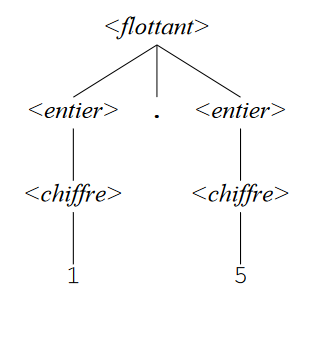
\includegraphics[width=0.10\textwidth]{expression1point5.png}
        \end{center}
    \end{figure}

    \paragraph{Grammaires ambigues}
    Une grammaire est \textbf{ambigue} ssi il existe une phrase dans $L(G)$ qui
    a plusieurs arbres de dérivations. 

    \begin{EExample}{Phrase ambigue}{}
        \begin{align*}
            \langle \texttt{expr} \rangle  &\Coloneqq x \\
            \langle \texttt{expr} \rangle &\Coloneqq \langle \texttt{expr}   \rangle - \langle \texttt{expr}   \rangle
        \end{align*}
    \end{EExample}

    \begin{figure}[H]
        \begin{center}
            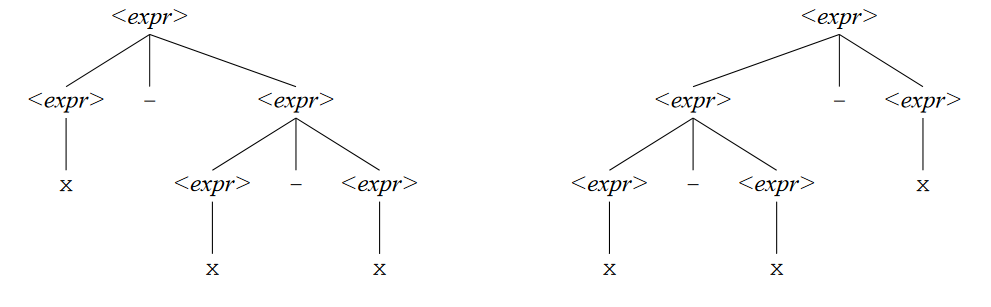
\includegraphics[width=0.30\textwidth]{GrammaireAmbig}
        \end{center}
    \end{figure}

    \paragraph{Autres motifs de syntaxes BNF}
    \begin{align*}
        &x_1 | x_2 : \textit{peut être} x_1 \textbf{ou} x_2 \\ 
        &(x) : \textit{groupement} \\ 
        &[x] \;\; \textbf{ou} \;\; x? \;\; \textbf{ou} \;\; \varepsilon| x : 
        x \textit{ peut apparaître  } \textbf{0} ou \textbf{1} \textit{ fois} 
        \\
        &\{x\} \;\; \textbf{ou} \;\; : x \;\; \textit{peut être répété } \textbf{ 0} 
        \textit{ou} \textbf{ plusieurs} \textit{ fois}         
    \end{align*}

    \begin{figure}[H]
        \begin{center}
            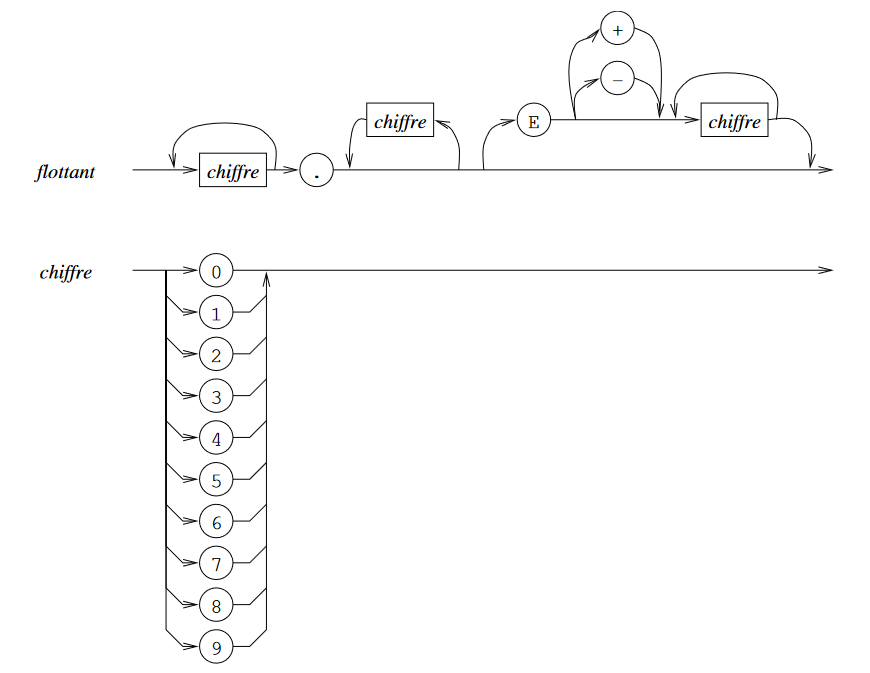
\includegraphics[width=0.25\textwidth]{diagrammesyntaxique}
        \end{center}
    \end{figure}

    \paragraph{Sucre syntaxique}
    \begin{itemize}
        \item [$\rhd$ ] Exension syntaxique superficielle \textbf{équivalente} à 
            une autre syntaxe 
        \item [$\rhd$ ] Pas d'impact sur les propriétés internes du langage
    \end{itemize}

    \paragraph{Langage fonctionnel}
    Les langages \textbf{fonctionnels} fournissent une environnment pour générer
    du code à un haut niveau d'abstraction. Le programmation fonctionnelle est
    un paradigme de programmation pour laquelle les expressions sont plus
    importantes que les affirmations. On compose ainsi les programmes en
    utilisant des \textbf{expressions}; chacune d'elles génère une valeur et ces
    expressions peuvent être combinées pour engendrer une expression plus
    complexes. Cette approche est différente de la programmation impérative où
    les affirmations ont un effet sur l'état global et où les affirmations
    communiquent des valeurs via l'état global. 
    
    \chapter{Lambda calcul}
    Le calcul lambda décrit comment \textit{définir} des fonctions et comment les 
    appeler.
    \paragraph{Syntaxe}
    \begin{align*}
          \lambda \textcolor{blue}{x}\textcolor{myp}{.} 
          \textcolor{red}{x} + 2    
    \end{align*}
    \begin{itemize}
      \item [$\rhd$] $\lambda$ : On déclare la \textbf{création} d'une fonction  
      \item [$\rhd$] $\textcolor{blue}{x}$ : Déclare la \textbf{variable}
        dépendante de la $f$ 
      \item [$\rhd$] $\textcolor{myp}{.}  $ : Sépare les déclarations de l'expression 
      \item [$\rhd$] $\textcolor{red}{x} + 2$ : Expression définissant $f$  
    \end{itemize}

    \begin{align*}
        (\lambda x. x + 2) \; 3 \leftrightarrow \; f(3)
    \end{align*}


    \begin{itemize}
      \item [$\rhd$] On appelle la $f$ avec l'argument \textbf{3}  
      \item[$\blacktriangleright$] Logiquement équivalent à $f(3)$
    \end{itemize}

    \begin{Concept}{}{}
        Puisque les fonctions acceptent des \textbf{valeurs}; on peut 
        passer des fonctions comme valeur dans d'autres fonctions, comme 
        lorsqu'on effectue une composition $f \circ g$
    \end{Concept}

    \begin{Definitionx}{Termes lamda}{}
        Une \textbf{fonction} est une expression lamda; elle est composée 
        de trois \textbf{types} de \textit{termes lambda} fondamentaux    
    \end{Definitionx}

    \paragraph{Termes lambda}

    \begin{itemize}
      \item [$\rhd$ ] \textbf{Variable}, p. ex. \textcolor{blue}{$x$}  
      \item [$\rhd$ ] \textbf{Fonction}, p. ex. 
        $\lambda$\textcolor{blue}{$x$}\textcolor{myp}{$.$}\textcolor{red}{$x$} +
        2        $\leftrightarrow$ $f(x) = x + 2$ 
      \item [$\rhd$ ] \textbf{L'expression d'appel}; \textit{calling a function}  
      \item [$\blacktriangleright$ ] p. ex $(\lambda x.x+2)y$ $\leftrightarrow$ $f(y)$

    \end{itemize}

    \begin{note}{}{}
      L'utilisation de \textbf{parenthèse} dans $(\lambda x.x+2)y$ 
      permet d'identifier
        et de distinguer
        la variable ($x$) de l'expression de la fonction et la viriable 
        ($y$) utilisée pour l'appel
    \end{note}

    \paragraph{Simplification d'expression}
    Il existe des règles qui permettent de simplifier les expressions 
    lambda et ainsi effectuer des calculs de fonction. Ces règles 
    sont analogues aux règles utilisée pour simplifier des expressions 
    algébriques

    \paragraph{Règle 1}
    \mbox{}\\
    \textit{Le nom d'une fonction n'a pas d'importance}.  
    \begin{align*}
        \lambda x.x+2 \leftrightarrow \lambda y.y+2
    \end{align*}

    \paragraph{Règle 2}
    \mbox{}\\
    \textit{On calcule une fonction en substituant la paramètre d'entrée 
    définissant la fonction avec le terme d'entrée présenté pour le calcul}
    \begin{align*}
         (\lambda x.\textcolor{red}{x}  +2)\textcolor{blue}{5}   
          \leftrightarrow f(\textcolor{blue}{5}  ) = \textcolor{red}{5} + 2  
    \end{align*}

    \paragraph{Syntaxe d'expression}
    En lambda calcul, chaque composante d'une expression est 
    aussi une expression (E). Et chaque expression doit satisfaire 
    la syntaxe suivante. 
    \mbox{} \\\\
    \begin{align*}
      & E \rightarrow \text{ID} \\
      & E \rightarrow \lambda \; \text{ID } . \; E \\ 
      & E \rightarrow E \; E \\
      & E \rightarrow (E) 
    \end{align*}
    Certaines expressions telles que $\lambda x. y z$ sont ambigue; 
    il faut donc des règles de disambiguation. 

    \paragraph{Règles de disambiguation} \mbox{}\\ 
    $\rhd$ $E \rightarrow E \; E$ est associatif à gauche

    \begin{align*}
        & x y z \leftrightarrow (x y)z \\ 
        & w x y z \leftrightarrow ((w x) y) z
    \end{align*}

    \noindent
    $\rhd$ $\lambda \text{ ID} \; . \; E$ s'étend à droite autant 
    que possible, commençant part $\lambda \text{ ID}$

    \begin{align*}
        & \lambda x \;. \; x y \leftrightarrow \lambda x \; . \; (x y) \\
        & \lambda x \;. \; \lambda x \;. \;x 
        \leftrightarrow \lambda x \; . \; (\lambda x \; . \; x) \\ 
        & (\lambda x \; . \; x y) z \leftrightarrow 
        (\lambda x \; . \; (x y)) \\ 
        & (\lambda x \; . \; w x y) z  \leftrightarrow 
        (\lambda x \; . \; ((w x) y)) z \\ 
        & \lambda x \; . \; (x) \leftrightarrow \lambda x \; . ((x) y) \\ 
        & \lambda a \; . \; \lambda b \; . \; \lambda c \; . \; 
        a b c \leftrightarrow 
        \lambda a \; . \; (\lambda b \; . \; (\lambda c \; . \; ((a b) c)) )
    \end{align*}


    \paragraph{Sémantique} \mbox{}\\
    $\rhd$ En lambda calcul, un ID tel que décrit par les règles de 
    syntaxe est en fait une \textbf{variable}.   
    \mbox{} \\\\ 
    $\rhd$ $ E \rightarrow \lambda \; \text{ID} \; . \; E$ est une 
    \textbf{abstraction} et l'ID est la \textbf{variable} 
    de l'abstraction. La seconde entité $E$ est le \textbf{corps} de 
    l'abstraction.     
    \mbox{}\\\\
    $\rhd$ $ E \rightarrow E \; E$ est une \textbf{application}  
    \mbox{} \\\\  
    $\rhd$ $ \lambda \; \text{ID} \; . \; E$ \textbf{définit} une nouvelle 
    fonction anonyme
    \mbox{} \\ 
    $\rhd$ $E \rightarrow E_1 \; E_2$ correspond à \textbf{l'appel de la 
    fonction} $E_1$ en établissant $E_2$ comme sont paramètre formel 

    \begin{EExample}{Fonction incrément}{}
        $$\lambda x \; . \;  + x \; 1$$ 
        Représente une fonctioon qui ajoute 
        \textbf{1} à son argument.   
        $$(\lambda x \; . \;  + x \; 1) \; 2$$  
        Représente l'appel ou \textit{application} de cette fonction 
        en établissant 
        \textbf{2} comme étant paramètre formel.   
        $$(\lambda x \; . \;  + x \; 1) \; 2 = 2 + 1 = 3$$ 
        Or, la fonction suivante ne peut pas être calculée lorsqu'elle 
        est appelé avec \textbf{2}  :
        $$\lambda y \; . \;  + x \; 1$$ 
        En effet, l'application de la fonction correspond à la substitution 
        de tous les '$y$' du corps de l'expression par le pamètre formel
        \textbf{2}. Mais le corps de l'expression définit un fonction 
        en termes de $x$ et non $y$; la substitution ne peut donc pas 
        se faire et l'évaluation de la fonction avec \textbf{2} se réduit 
        uniquement à $x + 1$ : 
        $$(\lambda x \; . \;  + x \; 1) \; 2 = x + 1 $$ 

        \end{EExample}


    \paragraph{Currying}
    Il s'agit d'une technique pour traduire l'évaluation d'une fonction 
    qui prend multiples arguments en une séquence de fonctions 
    qui prennent chacune un \textbf{unique} argument.   

    \begin{EExample}{}{}
        \begin{align*}
          \lambda x \; . \; \lambda y \; . \; ((+ x) y)
        \end{align*}
        Est composé de deux \textbf{abstractions}. L'abstraction externe 
        introduite par $\lambda x$ suggère qu'on doit substituer le 
        paramètre formel là où le reste de l'expression contient 
        la variable $x$. Ainsi, l'appel de fonction suivant peut être 
        réduit : 

        \begin{align*}
          \bigl(\lambda x \; . \; \lambda y \; . \; ((+ x) y)\bigr) 1
          =
          \lambda y \; . \; ((+ \; 1)y) 
        \end{align*}
    \end{EExample}


      \begin{EExample}{Addition par currying}{}
         \begin{align*}
            \bigl( \lambda x \; . \; \lambda y \; . \; ((+ \; x) \;y)\bigr)
            \; 10 \; 20 &= \bigl( \lambda y \; . \; ((+ \; 10)) \; y \bigr) 
            \; 20 \\ 
                    &= (+ \; 10) \; 20 \\          
                    &= 10 + 20 \\
                    &= 30 
          \end{align*}
      \end{EExample}


  \begin{Definitionx}{Variable libre}{}
      Dépendamment de la portée d'une expression, une variable peut être 
      lié \textit{bound} à une abstraction si la variable de l'abstraction 
      correspond à cette variable. On dit qu'un variable est libre 
      lorsqu'elle ne correspond pas à la variable ID de l'abstraction 
      mais apparaît quand même dans l'expression de cette abstraction. 

      $$ \lambda x \; . \; (+ 1) \; y  $$
      Est une abstraction qui contient la \textbf{variable libre} 
      $y$ puisque l'abstraction est exprimé en terme de $y$, alors 
      que $\lambda$ est suivit de la métavariable $x$. 
  \end{Definitionx}

  \begin{EExample}{Identification de variable libre}{}
    \begin{align*}
      \lambda x \; . \; x y z : \textbf{pour } x \text{ ?}  
    \end{align*}
    Non, puisque $x$ apparaît dans l'expression de l'abstraction 
    et que l'abstraction contient de métavariable $x$; $x$ est lié 
    à la fonction. 

    \begin{align*}
      \lambda x \; . \; x y z : \textbf{pour } y \text{ ?}                 
    \end{align*}
    Oui, $y$ n'est pas la métavariable de l'abstraction. 
      

    \begin{align*}
      (\lambda x \; . \; (+ \; x \; 1)) \; x : \textbf{pour } x \text{ ?}  
    \end{align*}

    Le premier $x$ est à l'intérieur d'une abstraction qui a 
    une métavariable du même nom. Le second $x$ est un paramètre formel 
    utilisé pour évaluer l'expression de l'abstraction et est donc 
    une variable libre. 

    \begin{align*}
      \lambda x \; . \; \lambda y \; . \; \lambda z \; . \; 
      z y x : \textbf{pour } z \text{ ?}  
    \end{align*}

    Non, puisque $z$ apparaît dans l'expression  et a la même 
    identité que la métavariable de l'abstraction. 

    \begin{align*}
      (\lambda x \; . \; z \; \texttt{foo})   (\lambda y \; . \; y x) 
     : \textbf{pour } x \text{ ?}  
    \end{align*}

    Oui, puisque $x$ n'apparaît pas dans le corps de la première 
    expression, malgré l'existance de la métavariable $x$. 
    Et pour la seconde expression, la métavariable est $y$; 
    le $x$  qui apparaît dans le corps de cette expression 
    n'est donc pas lié à la métavariable de l'expression.  
  \end{EExample}

    \paragraph{Règles d'expression libre}
    La variable $x$ est \textbf{libre} dans 
    une expression $E$ \textbf{Si} :    
    \begin{align*}
      & E = x \\
      & E = \lambda y \; . \; E_1, \text{où } y!= x \text{ et } x 
      \text{  libre dans } E_1 \\
      & E = E_1 E_2, \text{où } x  \text{est libre dans } E_1 \\
      & E = E_1 E_2, \text{où } x  \text{est libre dans } E_2
    \end{align*}

    La première règle dit que si l'expression est simplement la 
    variable $x$, $x$ est libre dans cette expression. 
    La seconde règle dit que si $x$ est libre dans une expression 
    E si $x$ est libre dans l'abstraction interne $E_1$, 
    tant que la métavariable 
    de l'abstraction externe n'est pas équivalente à $x$
    Les deux dernières règle indiquent que $x$ est libre dans une 
    expression $E$ composée de deux expression $E_1$ $E_2$, tant 
    que $x$ est libre dans une de ces deux expressions.


    \begin{EExample}{Variable libre}{}
        Est-ce que $x$ est libre dans les expression suivantes :
        \begin{align*}
          x \lambda x \; . \; x 
        \end{align*}
      Oui, puisque l'expression désambiguié est 
      $x (\lambda x \; . \; x)$ et obéit à la syntaxe 
      $E \rightarrow E_1 E_2$  où $x$ de $E_1$ est tel que 
      $E_1 = x$ et est donc une variable libre. Ainsi 
      l'expression globale $E = E_1 E_2$ est libre puisque 
      $x$ est libre dans $E_1$. 
        \begin{align*}
          \lambda x \; . \; y x
        \end{align*}
      Non puisque $x$ fait parti de corps de l'abstraction; 
      la métavariable de l'abstraction est aussi $x$, donc $x$ n'est pas 
      libre dans cette expression.
    \end{EExample}

    \begin{Definitionx}{Combinateur}{}
        Une expression est un combinateur si elle ne contient aucune 
        variable libre.  
    \end{Definitionx}

    \begin{EExample}{}{}
        \begin{align*}
          \lambda x \; . \lambda y \; . \; x y x 
        \end{align*}
        Est un combinateur, puisque $y$ est lié à l'abstraction interne 
        et $x$ est lié à l'abstraction externe
        \begin{align*}
          \lambda x \; . \; x 
        \end{align*}
        Est un combinateur puisque $x$ est lié à l'abstraction dont 
        la métavariable a la même idendité
        \begin{align*}
          \lambda z \; . \; \lambda x \; . \; x y z
        \end{align*}
        N'est pas un combinateur, puisque $y$ n'est pas lié
    \end{EExample}


    \begin{Definitionx}{Variable liée}{}
        Une variable liée est une variable qui n'est pas libre. Lorsqu'une 
        variable est liée, il important de déterminer à quelle abstraction 
        elle est liée.
    \end{Definitionx}


    \begin{note}{}{}
        Les variables \textbf{libres} et \textbf{liées} en programmation 
        fonctionnelle se comportent 
        comme les variable globales et locales dans les langages 
        impératifs. Lorsqu'un variable est libre dans une fonction interne 
        il est possible qu'elle soit tout de même lié à une abstraction 
        externe. 
    \end{note}

    \begin{EExample}{}{}
        L'expression suivante s'évalue comme suit
        \begin{align*}
          (\lambda x \; . \; x (\lambda x \; . \; x)) 1
          &= 1 (\lambda x \; . \; x)
        \end{align*}
        Seul le premier $x$ de l'expression a été substitué pour 
        l'argument $1$, puisque seul ce $x$ est lié à l'abstraction externe. 
        Le second $x$ est lié à l'abstraction interne. 
        \\\\ 
        On peut aussi considérer le corps de l'abstraction externe :
        \begin{align*}
            x (\lambda x \; . \; x)
        \end{align*}

        Dans cette expression, ($E \rightarrow E_1 E_2$), on a 
        $E_1 = x$ et donc le premier $x$  est une variable libre. 
        Sachant que le premier $x$ est une variable libre, on peut déduire 
        que ce $x$ est lié à une de niveau supérieur (abstraction externe),
        pourvue que cette abstraction contient la métavariable $x$. 
    \end{EExample}


    \paragraph{Equivalence}

    \begin{Definitionx}{$\alpha$-equivalence}{}
        Deux fonctions sont alpha équivalentes lorsqu'elles 
        diffèrent uniquement pas le nom des \textbf{variables liées}  
        \begin{align*}
          E_1 =_\alpha E_2
        \end{align*}
    \end{Definitionx}

    \paragraph{Opérations de renommage}
    On utilise la syntaxe $E\{ y \; /\ x \}$ pour signifier 
    qu'on \textbf{substitue} toutes les instances de $x$ par $y$ 
    dans l'expression $E$. La substitution doit obéir au règles suivantes 
    \mbox{}
    \\\\
    $E \{ y  \; /\ x\}$ \textbf{:}  
    \begin{align*}
      & x \{ y \; /\ x \} = y 
      \\ 
      & z \{ y \; /\ x \} = z \textbf{ si } z \neq x 
      \\   
      & (E_1 E_2) \{ y \; /\ x \} = 
          (E_1 \{ y \; /\ x \}) 
          (E_2 \{ y \; /\ x \}) 
          \\ 
      & \lambda x \; . \; E \{ y \; /\ x \} = 
        \lambda y \; . \; E \{ y \; /\ x \} 
        \\ 
      & \lambda z \; . \; E \{ y \; /\ x \} = 
        \lambda z \; . \; E \{ y \; /\ x \} 
        \textbf{ si } z \neq x   
    \end{align*}
  \begin{EExample}{Substitutions}{}
      \begin{align*}
        \lambda x \; . \; x \{ \texttt{foo} \; /\ x  \}
        &=
        \lambda \texttt{foo} \; . \; x \; \{ \texttt{foo} \; /\ x  \} \\
        &=
        \lambda \texttt{foo} \; . \;  \texttt{foo}    
      \end{align*}

      \begin{align*}
        &(\lambda x  \; . \; x (\lambda y \; . \; x y z y) x y)   
        \; \{ \texttt{bar} \; /\ x  \}
        \\
        &= 
        \lambda \texttt{bar} \; . \; 
        \bigl( x (\lambda y \; . \; x y z y) x y\bigr) 
          \{\texttt{bar} \; /\ x \}
         \\
        &=
        \lambda \texttt{bar}  \; . \; \texttt{bar}  
        \bigl(\lambda y \; . \; x y z y\bigr) x y \; 
          \; \{\texttt{bar} \; /\ x \}
        \\
        &=
        \lambda \texttt{bar}  \; . \; \texttt{bar}  
        \bigl(\lambda y \; . \; x y z y \{\texttt{bar} \; /\ x   \} \bigr)
        \bigl( x y \; \{\texttt{bar} \; /\ x \} \bigr) \\
        &= 
        \lambda \texttt{bar} \; . \; \texttt{bar}
        \bigl(\lambda y \; . \; \texttt{bar}yzy   \bigr)
        \bigl( \texttt{bar} y \bigr)
      \end{align*}
  \end{EExample}

  \begin{Theorem}{Expressions $\alpha$-équivalentes}{}
      Tant que la varable $y$ n'appartient pas à l'expressions 
      $E$, toutes les expression $\lambda y \; . \; E \{ y \; /\ x \}$ 
      sont alpha équivalentes à l'expression $\lambda x \; . \; E$

      \begin{align*}
        \lambda x \; . \; E =_{\alpha} \lambda y \; . \; E \{y \; /\ x \}
        \big| \; y \notin E
      \end{align*}
  \end{Theorem}

  \paragraph{Opération de substitution} 
  Le \textbf{renommage} permet uniquement de remplacer une variable 
  par une autre $(\{ x \; /\ y \})$. Or, pour réduire une 
  expression, il faut effectuer une \textbf{substitution}  

  \begin{align*}
    E[x \rightarrow N] \ ; \Big| \; E = E_1, N = E_2 
    \text{ sont des } \lambda\text{-exp}.
  \end{align*}

  Cette expression revient à dire qu'on remplace $x$ avec 
  $N$ où $E$ et $N$ sont des $\lambda$-expressions et $x$ est 
  une \textbf{variable non liée}  . 

  \begin{EExample}{}{}
     \begin{align*}
        & (+ \; x \; 1) [x \rightarrow 2] = ( + \; 2 \; 1) \\
        & (\lambda x \; . \; + \; x \; 1) [x \rightarrow 2] 
        = (\lambda x \; . \; + \; x \; 1) \\
        & (\lambda x \; . \; y \; x) [y \rightarrow \lambda z \; . \; x z]  \\
        &= \\
        & (\lambda x \; . (\lambda z \; . \; x z) x) \; \textbf{Intermédiare}
        \\
        &= 
        \\
        & (\lambda w \; . (\lambda z \; . \; x z) w) \\ 
     \end{align*} 
  \end{EExample}

  \paragraph{Règles de substitution}
  \begin{align*}
    & x [ x \rightarrow N] = N \\ 
    & y [ x \rightarrow N] = y \textbf{ si } x \neq y   \\ 
    & (E_1 \; E_2) [ x \rightarrow  N] = 
    \bigl( E_1 \; [x \rightarrow N]\bigr) 
    \bigl( E_2 \; [x \rightarrow N]\bigr) \\ 
    & \lambda x \; . \; E [ x \rightarrow N] = \lambda x \; . \; E \\ 
    & \lambda y \; . \; E [ x \rightarrow N] = 
    \lambda y \; . \; \bigl( E[x \rightarrow N] \bigr) 
    \\
    &\texttt{où } x \neq y \text{, et }
    y \text{ n'est pas libre dans } N 
    \\ 
    & \lambda y \; . \; \bigl( E[x \rightarrow N] \bigr) 
    =
    \bigl( \lambda y^{\prime} \; . \; 
    E \{y^{\prime} \; /\ y \}[x \rightarrow N]\bigr)
    \\ 
    &\texttt{où } x \neq y, y \text{ libre dans } N \text{, et } \\
    &y^{\prime} \text{ est un nouveau nom}
  \end{align*}

  \begin{EExample}{}{}
      \begin{align*}
        & (\lambda x \; . \; x) [x \rightarrow \texttt{foo}  ] 
        = 
        (\lambda x \; . \; x)
        \\
        & \text{Obéit à } \lambda x \; . \; E [x \rightarrow N] 
        = 
        \lambda x\; . \; E
      \end{align*}

      \begin{align*}
        & (+ \; 1 \; x)[x \rightarrow 2] 
        \\
        &= 
        \bigl(((+ \; 1) \; x) [x \rightarrow 2] \bigr) 
        \bigl( x [x \rightarrow 2] \bigr)  \\
        & \text{Obtéit à} 
        (E_1 \; E_2) [x \rightarrow N]
        \\
        &= 
        (E_1 [x \rightarrow N]) \; (E_2 [x \rightarrow N])\\
        &\leftrightarrow 
        \bigl(+ [x \rightarrow 2] \bigr)         
        \bigl(1 [x \rightarrow 2] \bigr)         
        \bigl(x [x \rightarrow 2] \bigr) \\ &= + (\; 1 \; 2)
      \end{align*}

      \begin{align*}
        &(\lambda x \; . \; y x)[y \rightarrow \lambda z \; . \; x z]
        \\
        &= 
        \lambda w \; . 
        \bigl(\; y x\bigr) \{ w \; /\ x \}
        [y \rightarrow \lambda z \; . \; x z]
        \\ 
        &= \lambda w \; . \; \bigl( yw \bigr)
        [y \rightarrow \lambda z \; . \; x z]
        \\ 
        &= \lambda w \; . \; 
        \bigl( y 
        [y \rightarrow \lambda z \; . \; x z]\bigr)
        \bigl(w [y \rightarrow \lambda z \; . \; x z] \bigr)
        \\ 
        &= \lambda y \; . \; 
        (\lambda z \; . \; xz) (w)
      \end{align*}
  \end{EExample}

  \paragraph{Execution}
  \mbox{}
  \vspace{0.5em}

  \begin{Definitionx}{Exécution}{}
      Engendre une séquence de termes qui est le résultat 
      d'appels et d'invocations de fonctions
  \end{Definitionx}

  \noindent
  $\rhd$ Chaque étape du processus d'\textbf{exécution} 
  est appelé $\beta$-reduction. 
  \mbox{}\\ \\
  $\rhd$ On peut seulemnet $\beta$-réduire des 
  \textbf{$\beta$}-redux; des expressions sous la forme 
  \textit{application}  
  \begin{itemize}
    \item [$\blacktriangleright$ ] $(\lambda x \; . \; E) \; N$
  \end{itemize}
  \mbox{}\\
  $\rhd$ Une $\beta$-réduction est définit par :
  \begin{align*}
      (\lambda x \; . \; E) \; N 
      \text{ se } \beta\text{-réduit à } E[x \rightarrow N]
  \end{align*}



  \begin{EExample}{Exécutions}{}
    \textbf{Exercice 1} :  
      \begin{align*}
        (\lambda x \; . \; x) y 
        &= x[x \rightarrow y] = y
      \end{align*}

    \textbf{Exercice 2} :
      \begin{align*}
      &\bigl( \lambda x \; . \; x (\lambda x \; . \; x) \bigr) u r
      \\
      &= \Bigl(\bigl( \lambda x \; . \; x (\lambda x \; . \; x) \bigr) u\Bigr) r
      \\
      &= \Bigl(  x (\lambda x \; . \; x)[x \rightarrow u] \Bigr) r
      \\
      &= \Bigl(  \bigl(x[x \rightarrow u]\bigr) 
          \bigl(\lambda x \; . \; x)[x \rightarrow u]\bigr) \Bigr) r
      \\
      &= \Bigl(u \; \lambda x \; . \; x \Bigr) r
      \end{align*}

    \textbf{Exercice 3} : 
      \begin{align*}
       &\bigl( \lambda x \; . \; x (\lambda x \; . \; x) \bigr) (u r) 
       \\
       & = x (\lambda x \; . \; x)[x \rightarrow (u r)]
       \\
       & = \bigl(x [x \rightarrow (u r)] \bigr)
           \bigl(\lambda x \; . \; x [x \rightarrow (u r)] \bigr)
        \\ 
       & = (u r)(\lambda x \; . \; x)
      \end{align*}
  \end{EExample}  

  \paragraph{Logique booléenne}
  \mbox{}\\\\
  \noindent
  $\rhd$ \texttt{True} est une \textit{fonction} qui prend deux argument 
  et retourne le \textbf{premier}   
  \begin{align*}
    T = \lambda x \; . \; \lambda y \; . \; x 
  \end{align*}

  \noindent
  $\rhd$ \texttt{False} est une \textit{fonction} qui prend deux argument 
  et retourne le \textbf{second}   
  \begin{align*}
    F = \lambda x \; . \; \lambda y \; . \; y 
  \end{align*}

  \begin{EExample}{}{}
    \begin{align*}
      (\lambda x \; . \; \lambda y \; . \; x) \; a \; b
      &= 
      ((\lambda x \; . \; \lambda y \; . \; x) \; a) \; b
      \\
      &= 
      \bigl((\lambda y \; . \; x)[x \rightarrow a]\bigr) b 
      \\ 
      &= \bigl( \lambda y \; . \; a \bigr) b
      \\
      &= \bigl( \lambda y \; . \; a \bigr)[y \rightarrow b]
      \\ 
      &= a
    \end{align*} 
  \end{EExample}
  \mbox{}\\
  
  \noindent
  $\rhd$ \texttt{AND} est une \textit{fonction} qui prend deux arguments 
  et renvoit \texttt{True} lorsqu'ils sont tous deux \texttt{True} et 
  \texttt{False} autrement. 
  \begin{align*}
      \texttt{AND} = \lambda x \; . \; \lambda y \; . \; x y x  
  \end{align*}

  
    \paragraph{Cas 1: \(x = T\), \(y = T\)}

    \begin{align*}
    (\lambda x . \lambda y . x y x) \, T \, T &= (\lambda y . T \, y \, T) \, T \\
                                              &= T \, T \, T \\
                                              &= T
    \end{align*}

  \paragraph{Cas 2: \(x = T\), \(y = F\)}

  \begin{align*}
  (\lambda x . \lambda y . x y x) \, T \, F &= (\lambda y . T \, y \, T) \, F \\
                                            &= T \, F \, T \\
                                            &= F
  \end{align*}

  \paragraph{Cas 3: \(x = F\), \(y = T\)}

  \begin{align*}
  (\lambda x . \lambda y . x y x) \, F \, T &= (\lambda y . F \, y \, F) \, T \\
                                            &= F \, T \, F \\
                                            &= F
  \end{align*}

  \paragraph{Cas 4: \(x = F\), \(y = F\)}

  \begin{align*}
  (\lambda x . \lambda y . x y x) \, F \, F &= (\lambda y . F \, y \, F) \, F \\
                                            &= F \, F \, F \\
                                            &= F
  \end{align*}

  \mbox{} 
  \noindent 
  $\rhd$ \texttt{NOT} est une \textit{fonction} qui prend un argument 
  et renvoit l'opposé de celui-ci 

  \begin{note}{}{}
      Puisque l'argument de \texttt{NOT} est une fonction 
      \texttt{True} ou \texttt{False}, en principe, 
      \texttt{NOT} doit prendre deux arguments. 
      La fonction que prend \texttt{NOT} (l'argument de \texttt{NOT})
      renverra le premier argument si cette fonction est \texttt{True}
      La fonction que prend \texttt{NOT} renverra le second 
      argument si cette fonction est \texttt{False}. C'est pourquoi 
      dans le corps de l'expression \texttt{NOT} il y a deux fonctions, soit 
      \texttt{False} et \texttt{True} placées \textbf{devant} la fonction 
      qui sera substituée par $x$; ces fonctions servent d'argument 
      à la fonctione substuée par $x$, qui se trouve à être 
      l'argument de \texttt{NOT}.  
  \end{note}

  \begin{align*}
    \texttt{NOT} = \lambda x \; . \; x F T   
  \end{align*}


  \paragraph{Cas 1: \(x = T\)}
  \begin{align*}
    (\lambda x . x F \, T) T &= x \, F \, T[x \rightarrow T] \\
                                  &= T F T \\ 
                                  &= (\lambda x . \lambda y . x) F T \\ 
                                  &= (\lambda y . x )[x \rightarrow F] T \\
                                  &= (\lambda y . F) T \\ 
                                  &= (F [y \rightarrow T]) \\ 
                                  &= F
  \end{align*}


  \paragraph{Cas 2: \(x = F\)}
  \begin{align*}
    (\lambda x . x F \, T) T &= x \, F \, T[x \rightarrow F] \\
                                  &= F F T \\ 
                                  &= (\lambda x . \lambda y . y) F T \\ 
                                  &= (\lambda y . y )[x \rightarrow F] T \\
                                  &= (\lambda y . y) T \\ 
                                  &= (y [y \rightarrow T]) \\ 
                                  &= T
  \end{align*}

  \paragraph{Branche \texttt{if}}
  Les branches permettent de changer le flow d'exécution d'une programme, 
  en fonction de la condition du branchement et de la variable d'entrée. 

  \mbox{}\\ 
  \noindent 
  L'architecture d'une \textit{fonction} 
  \texttt{if}, en lambda calcul, devrait donc être telle que la fonction  
  prend un booléen, comporte une branche \texttt{True} et 
  comporte une seconde branche \texttt{False}.   


  \begin{lstlisting}
  if c then 
    a 
  else 
    b
  \end{lstlisting}

  Le squelette de la fonction serait : 
  \begin{align*}
    \texttt{if} \; c \, a \, b  
  \end{align*}
  La fonction \texttt{if} devrait retourner $a$ ou $b$, dépendamment 
  du booléen présenté en argument. La fonction \texttt{tx} prend alors 
  trois paramètres. Si le paramètre booléen est vrai, elle retourne 
  le paramètre $a$, qui se trouve à être le premier paramètre après le paramètre 
  booléens. Si le paramètre booléen est faux, elle retourne le second paramètre
  après le paramètre booléen, soit $b$. 

  \mbox{}\\ 
  On constate que le paramètre $c$ est simplement la fonction 
  \texttt{True} ou la fonction \texttt{False}. On a : 

  \begin{align*}
    &\texttt{if} \; T \, a \, b = a   \\
    &\texttt{if} \; F \, a \, b = b   
  \end{align*}

  Ainsi, la fonction \texttt{if} semble avoir la même sémantique que la 
  fonction identité $\lambda x \, . \, x$ qui retourne la valeur 
  d'entrée. 

  Ainsi, on a 
  \begin{align*}
     &\texttt{if} \; T \, a \, b \leftrightarrow 
     (\lambda w \, . \, w) \lambda x \, . \, \lambda y \, . \, x \; a \, b        
     \\
     &\textbf{et}
     \\
     &\texttt{if} \; F \, a \, b \leftrightarrow 
     (\lambda w \, . \, w) \lambda x \, . \, \lambda y \, . \, y \; a \, b        
  \end{align*}

  \paragraph{Church's nurmerals}  
  L'intuition derrière les nombre de Church est qu'un nombre 
  correspond au nombre de fois où une fonction quelconque $f$ 
  passé en argument sur la fonction du nombre est appliqué sur la 
  variable $x$

  \[
  \begin{aligned}
  0 &= \lambda f . \lambda x . x \\
  1 &= \lambda f . \lambda x . f \, x \\
  2 &= \lambda f . \lambda x . f \, (f \, x) \\
  3 &= \lambda f . \lambda x . f \, (f \, (f \, x)) \\
  4 &= \lambda f . \lambda x . f \, (f \, (f \, (f \, x))) \\
  \end{aligned}
  \]


  \begin{EExample}{}{}
    \begin{align*}
      4 \, a \, b &= \bigl(\lambda f . \lambda x . f( f( f( f x))) a \bigr) b
      \\ 
              &= \bigl(\lambda x . f( f( f( f x))) a \bigr)[f \rightarrow a] \; b 
      \\
              &= \bigl(\lambda x . a ( a ( a ( a x)))\bigr) \; b 
      \\
              &= \bigl( a ( a ( a ( a x)))\bigr)[x \rightarrow b] \; b 
      \\ 
              &= \bigl( a ( a ( a ( a b)))\bigr) 
    \end{align*}
  \end{EExample}

  \paragraph{Fonction successeur}
  
  \begin{align*}
     \texttt{succ} = \lambda n . \lambda f . \lambda x . f(n \, f \, x)
  \end{align*}

  La fonction successeur en lambda calcul, notée 
  \texttt{succ}, est utilisée pour ajouter 1 à un nombre de Church.
  En d'autres mots, La fonction prend un nombre de Church $n$
  comme entrée et renvoie en sortie un nouveau nombre de Church qui représente 
  $n + 1$. 


  \begin{EExample}{Successeur de 1}{}

  \begin{align*}
    &\bigl(\lambda n . \lambda f . \lambda x . f (n \, f \, x) \bigr) 1 
    \\
    &= 
    \bigl(\lambda n . \lambda f . \lambda x . f (n \, f \, x) \bigr) 
    (\lambda f . \lambda x . f \, x)
    \\ 
    &= 
    \lambda f . \lambda x . f \bigl((\lambda f . \lambda x . f \, x) \, f \, x\bigr) 
    \\
    &= 
    \lambda f . \lambda x . f \bigl((\lambda x . f \, x)[f \rightarrow f] \, x\bigr)
    \\ 
    &= 
    \lambda f . \lambda x . f \bigl(f \, x\bigr)
    \\
    &= 
    \lambda f . \lambda x . f (f \, x)
    \\
    &= 
    \lambda f . \lambda x . f (f \, x)
  \end{align*} 
  \end{EExample}


  \paragraph{Addition}
  La fonction d'addition prend deux paramètre et retourne 
  une fonction qui correspond au nombre de Church représentant la 
  somme des deux paramètres 

  \mbox{}\\\\
  \noindent 
  Cela peut être interprété comme appliquer $f$ $n$ fois à $x$, puis 
  appliquer ce résultat $f$ $m$ fois à ce résultat.

  \begin{align*}
    \texttt{add} = \lambda m . \lambda n . \lambda f . \lambda x . n \, f \; 
    (m \, x \, f)
  \end{align*}

  \begin{EExample}{Addition de 0 et 1}{}
   \begin{align*}
    &(\lambda n . \lambda m . \lambda f . \lambda x . n f (m f x)) \; 0 \, 1 \\
    &= (\lambda m . \lambda f . \lambda x . 0 f (m f x)) \; 1 \\
    &= \lambda f . \lambda x . 0 f (1 f x) \\
    &= \lambda f . \lambda x . (\lambda f . \lambda x . x) f (f x) \\
    &= \lambda f . \lambda x . (\lambda x . x)[x \rightarrow f x] \\
    &= \lambda f . \lambda x . x \\
    &= \lambda f . \lambda x . f x
    \end{align*}     
  \end{EExample}


  \paragraph{Multiplication}
$$\lambda n . \lambda m . m (add n ) 0 $$




  \begin{EExample}{Multiplication de 0 et 1}{}
     \begin{align*}
      &(\lambda n . \lambda m . m (\text{add} \, n) \, 0) \, 0 \, 1 \\
      &= (\lambda m . m (\text{add} \, 0) \, 0) \, 1 \\
      &= 1 (\text{add} \, 0) \, 0 \\
      &= (\lambda f . \lambda x . f x) (\text{add} \, 0) \, 0 \\
      &= (\lambda f . \lambda x . f x) (\lambda m . \lambda f . \lambda x . 0 f (m f x)) \, 0 \\
      &= (\lambda f . \lambda x . f x) (\lambda f . \lambda x . 0 f (0 f x)) \\
      &= (\lambda f . \lambda x . f x) (\lambda f . \lambda x . x) \\
      &= \lambda x . (\lambda f . \lambda x . x) x \\
      &= \lambda x . x \\
      &= \lambda f . \lambda x . x
    \end{align*}
  \end{EExample}

  \paragraph{$Y$-combinator}
  Le combinateur $Y$ est une fonction qui, à cause de sa structure particulière 
  parvient à s'autorépliquer lorsqu'un argument lui est appliqué. La fonction 
  résultante l'application $Y a$ est $Y Y a$, qui à son tour, engendre 
  $Y Y Y a$, puis $Y Y Y Y a$, ainsi de suite. 

  \begin{align*}
    Y = \bigl(\lambda y . \lambda x . y (x \, x \, y)\bigr)
        \bigl(\lambda y . \lambda x . y (x \, x \, y)\bigr)
  \end{align*}

  \begin{EExample}{}{}
   \begin{align*}
    &Y 
    \text{foo} = \lambda f . (\lambda x . f (x x)) (\lambda x . f (x x)) \\
    &\text{foo} \\
    &= (\lambda f . (\lambda x . f (x x)) (\lambda x . f (x x))) \text{foo} \\
    &= (\lambda x . \text{foo} (x x)) (\lambda x . \text{foo} (x x)) \\
    &= \text{foo} ((\lambda x . \text{foo} (x x)) (\lambda x . \text{foo} (x x))) \\
    &= \text{foo} (Y \text{foo}) \\
    &= \text{foo} (\text{foo} (Y \text{foo})) \\
    &= \text{foo} (\text{foo} (\text{foo} (Y \text{foo}))) \\
    &\vdots
  \end{align*}     
  \end{EExample}




    






 


    



    
    \end{multicols*}





\end{document}
